\chapter{系统总体设计}
\vspace{7pt}

在完成系统需求分析的基础上，本章进一步从宏观层面给出系统的总体设计方案。首先阐述前后端分离的软件架构，明确各层职责与技术选型；随后重点介绍基于RAG的需求拆解流程与基于LangGraph的多智能体协同工作流设计；接着给出数据库概念模型与物理表结构；最后说明人机交互中动态表单的双向状态机逻辑。上述设计共同构成了系统实现的技术蓝图。

\section{系统软件架构设计}

\subsection{前后端分离架构设计}

本系统采用前后端分离的软件架构模式。后端负责业务逻辑处理、人工智能模型调用与PlantUML图表渲染，前端负责用户交互、数据可视化与代码编辑器集成。前后端之间通过RESTful API进行数据交互，遵循关注点分离原则，使前后端能够独立开发、独立部署与独立扩展。

后端以FastAPI作为Web框架构建。FastAPI基于Python的异步编程特性，支持自动生成OpenAPI规范的接口文档，并提供了基于Pydantic的请求数据校验机制。这些特性在后端需要处理大量异步大语言模型调用的场景下尤为重要。FastAPI的原生异步支持允许在等待大模型响应期间不阻塞事件循环，从而提高了服务的并发处理能力。

在人工智能工作流编排层面，系统引入LangGraph框架构建多智能体协作状态机。LangGraph以有向状态图的形式组织多个大语言模型调用节点的执行顺序与数据流向。每个节点代表一个独立的建模推理步骤，节点之间通过共享状态池传递中间结果。LangGraph内置的内存检查点机制为系统实现断点暂停与人工确认提供了关键基础设施。

在检索增强生成层面，后端集成ChromaDB向量数据库和Sentence-Transformers文本嵌入模型。ChromaDB以嵌入式模式运行在应用进程中，负责存储需求文档分块后的语义向量并支持高效相似度检索。检索结果被注入到大语言模型的提示词中，有效缓解了长文档场景下的信息丢失问题。

在模板渲染层面，后端采用Jinja2模板引擎将建模数据转化为PlantUML图表代码。系统为用例图、类图和时序图分别设计了独立的Jinja2模板文件，模板接收从状态池中提取的结构化建模数据，按照PlantUML语法规范填充占位符，生成完整的图表代码。模板化的设计将数据与表示逻辑解耦，使得图表代码的生成规则可以独立维护。

在数据持久化层面，系统选用MySQL关系型数据库配合SQLModel对象关系映射框架。SQLModel结合了SQLAlchemy的数据操作能力和Pydantic的数据校验能力，使得数据库模型的定义与API数据模式的定义保持一致性。关系型数据库的选型保障了项目数据、模块数据和UML模型数据之间关联关系的完整性和查询效率。

前端采用Vue 3组合式API与Vite构建工具。组合式API通过响应式引用和组合函数提供了更灵活的组件逻辑组织方式，使得项目管理界面、建模工作区和代码编辑器等复杂交互组件的状态管理更加清晰。Element Plus组件库提供了统一的企业级界面风格。Monaco Editor作为PlantUML代码的编辑和展示组件，提供了语法高亮、代码折叠和自动补全等专业编辑功能。

系统的整体逻辑架构如图4.1所示。自顶向下分为用户层、服务层、AI推理层和基础设施层。用户层承载前端页面的所有可视化组件。业务层封装了UML生成、项目管理和文档解析等核心功能模块。AI推理层基于LangGraph编排多Agent协作流程，并通过统一的LLM服务接口调用DeepSeek大语言模型。基础设施层包含MySQL数据库、ChromaDB向量数据库和PlantUML渲染引擎。

% 图4.1 系统逻辑架构图
\begin{figure}[htbp]
    \centering
    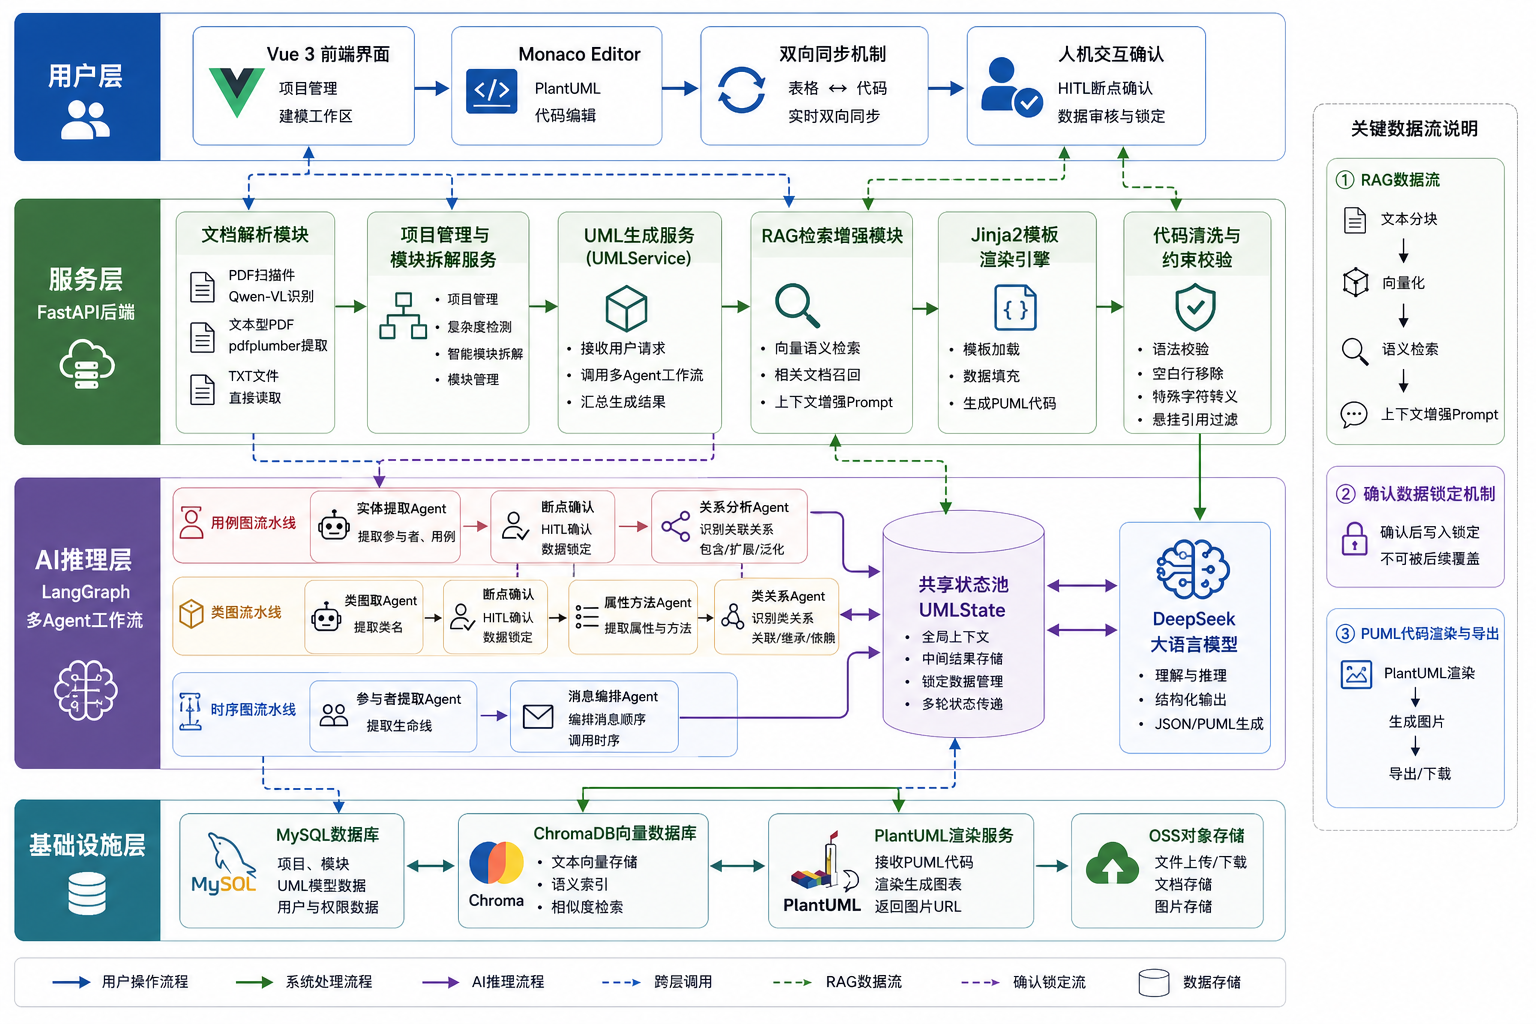
\includegraphics[width=150mm]{docs/imgs/系统架构图.png}
    % \vspace{-8pt}
    % \fontSimsun\sizeFive 图4.1 系统逻辑架构图
    % \vspace{-8pt}
    \caption{系统逻辑架构图}
    \label{fig:system_architecture}
\end{figure}

\section{核心算法工作流设计}

\subsection{基于RAG的需求拆解与模块管理流程设计}

检索增强生成技术在本系统中的第一个应用场景是复杂项目的需求拆解。当用户上传一份大规模的需求文档时，系统需要首先判断该文档是否包含多个功能模块，并自动将文档拆分为若干独立的建模单元。

在第一阶段，系统对原始需求文档进行文本分块。分块策略以句子边界为主要切分依据，在句号、问号、感叹号等自然语句结束符处进行分割。切分后的文本块通过paraphrase-multilingual-MiniLM-L12-v2嵌入模型转化为稠密语义向量。该嵌入模型是一个12层的多语言BERT变体，在保证语义表示质量的前提下具有较小的模型参数量和较快的推理速度。生成的向量连同原始文本块和元数据一起存入ChromaDB向量数据库中，形成项目的语义知识库。

在第二阶段，当系统需要对原始文档进行模块拆解时，根据不同的文档类型选择不同的处理路径。对于纯文本文档，系统直接调用大语言模型，在提示词中引导模型识别文档中描述的不同功能子系统，并为每个子系统提炼核心需求描述。对于PDF文档，系统首先将文档页面转换为图像，通过Qwen-VL视觉语言模型从图像中提取文字内容，同时获取文档的结构化信息。这一多模态解析能力使系统在处理扫描件PDF时无需依赖文字层，直接通过图像识别获取文本。

模块拆解完成后，系统为每个模块建立独立的建模空间，包括独立的thread\_id作为LangGraph工作流的会话标识。当用户针对某个模块启动用例提取任务时，RAG机制的第二重作用开始发挥。系统以该模块的需求描述文本作为查询，向ChromaDB发起语义检索请求。ChromaDB计算查询向量与所有已存储文档块向量的余弦相似度，返回相似度最高的若干段落作为检索结果。这些检索到的段落被格式化为上下文信息，拼接到发送给大语言模型的提示词开头。

通过这种上下文增强方式，模型在生成时不仅能看到当前模块的局部需求文字，还能参考原始需求文档中其他章节的相关描述。例如，当为“订单管理”模块生成用例图时，RAG可能检索到需求文档“用户管理”章节中关于用户角色权限的描述，以及“支付管理”章节中关于订单状态变更流程的描述。这些跨模块的信息有助于模型更准确地识别参与者角色和用例之间的依赖关系。

\subsection{基于LangGraph的多Agent协同设计}

LangGraph工作流的核心是UMLState状态池。状态池是一个类型化字典结构，定义了在多Agent协作过程中需要传递和共享的全部数据字段。状态池的设计遵循职责分离和信息聚合并重的原则，既为每种图表类型预留了专用的数据存储字段，又设置了跨图类型共享的基础字段。

状态池的基础字段包括当前模块的需求文本input\_text、用于RAG检索的原始整体需求original\_requirement、项目标识project\_id以及目标图表类型标识current\_diagram。用例图专用字段包括实体映射entities、角色列表actors、用例列表usecases、关系字典relationships，以及用于锁定的确认角色列表confirmed\_actors和确认用例列表confirmed\_usecases。类图专用字段包括实体类列表classes、类属性方法字典class\_details和类间关系字典class\_relationships。时序图专用字段包括选中用例列表selected\_usecases和时序数据字典sequence\_data。

工作流图的节点设计对应七类专业化Agent。每个Agent节点内部封装了对大语言模型的调用逻辑、提示词构建以及输出解析过程。Agent-1实体提取节点负责从需求文本中识别系统参与者和用例名称，输出结构化的实体映射。Agent-2关系分析节点负责推断参与者和用例之间的包含关系、扩展关系与泛化关系。Agent-3类实体提取节点负责识别需求文本中代表核心业务概念的实体类。Agent-4类属性方法提取节点负责分析每个实体类的属性和操作。Agent-5类关系分析节点负责判定类之间的关联、聚合、组合、继承和依赖关系。Agent-6时序参与者提取节点负责确定每个用例交互过程涉及的对象及其类型划分。Agent-7时序消息编排节点负责组织参与者之间的消息传递序列。

工作流图的边定义了节点间的执行顺序和数据流转方向。系统通过条件边实现工作流的路由分发。条件边的路由函数依据状态池中的current\_diagram字段值判定目标图表类型，将执行权导向对应的处理流水线。用例图流水线的执行顺序为实体提取节点后接关系分析节点。类图流水线的执行顺序为类实体提取、类属性方法提取和类关系分析三个节点依次执行。时序图流水线的执行顺序为时序参与者提取节点后接时序消息编排节点。每条流水线的终点均指向图结束。

断点机制是实现人机协同的核心设计。系统在LangGraph工作流编译时通过interrupt\_before参数指定了两个断点位置。第一个断点位于关系分析节点之前，即实体提取节点执行完成后工作流自动暂停，将提取出的角色和用例列表返回给前端界面展示，等待用户审查确认。第二个断点位于类属性方法提取节点之前，即类实体提取节点完成后暂停，等待用户确认类名列表。断点位置的选择基于建模任务的内在逻辑依赖。关系分析的正确性高度依赖于实体提取的完整性，因此需要在开始关系推理前让用户有机会修正实体列表。类属性方法提取同样依赖于类名的准确确定，在实际运行中，模型可能遗漏某些类或错误地将非实体概念识别为类，因此类名列表也需要在进入属性提取阶段前得到人工确认。

在多Agent协同中，还设计了锁定约束机制以防止后续Agent污染用户已确认的数据。当用户在前端确认了角色列表后，confirmed\_actors字段被写入状态池，实体提取节点在后续调用时将直接返回已确认的列表，不再接受模型新增实体。同样地，confirmed\_classes字段确保类提取节点不再新增类名，confirmed\_usecases字段锁定用例列表。这一锁定机制保证了用户的人工判断具有最终权威，避免了自动化流程与人工修正之间的冲突。

\section{数据库设计}

\subsection{概念模型设计}

系统的数据库概念模型围绕项目、模块和UML模型三个核心实体展开。项目实体代表一个完整的建模任务，是数据组织的顶层容器。每个项目包含名称、需求文本、是否为复杂项目、原始文件存储地址及LangGraph工作流会话标识等属性。模块实体是复杂项目下的子划分单元，每个模块属于一个项目，包含模块名称、描述、核心需求文本及独立的LangGraph会话标识。UML模型实体存储每次建模生成的结果，包含模型类型、结构化数据、PlantUML代码、渲染后的图片地址及确认状态标识。一个项目可以拥有多个模块，每个模块和每个项目均可关联多份UML模型记录。实体之间的参照完整性通过外键约束保证，项目删除时级联删除其下属的所有模块和UML模型记录。

\subsection{物理模型设计}

基于概念模型，系统设计了三张核心数据表。projects表作为项目主表，包含id主键、name项目名称、requirement\_text需求文本长文本字段、is\_complex布尔标志、original\_file\_url原始文件存储地址、thread\_id会话标识、description项目描述以及created\_at和updated\_at时间戳。thread\_id为每个项目分配唯一的UUID，作为LangGraph状态图的会话标识符，在多次API调用之间保持状态的连续性。

project\_modules表存储复杂项目的模块数据，包含id主键、project\_id外键、module\_name模块名称、description模块描述、core\_requirements模块核心需求长文本字段和thread\_id模块级会话标识。模块级thread\_id使每个模块拥有独立的LangGraph工作流上下文，用户在切换建模模块时，各模块的提取结果和确认状态互不干扰。

uml\_models表存储UML模型的生成结果，采用多类型统一存储的设计。表结构包含id主键、project\_id外键、module\_id可空外键、model\_type模型类型枚举字段、data\_json存储结构化数据的JSON字段、puml\_code存储PlantUML代码的长文本字段、image\_url渲染图片地址、usecase\_name时序图用例名称字段以及is\_confirmed确认状态布尔字段。时序图的每条记录对应一个用例，usecase\_name字段用于区分同一模块下不同用例的时序图。当module\_id为空时表示该模型记录属于项目级别而非模块级别，这一设计使系统同时支持简单项目的整体建模和复杂项目的分模块建模。

\section{人机交互设计}

人机交互层的数据流转遵循一个双向状态机逻辑。在多Agent工作流暂停于断点时，前端接收到包含角色、用例或类名列表的中间态JSON数据。这些数据通过Vue 3的响应式绑定渲染为可编辑的数据表格。表格的每一行代表一个提取结果，用户可以在表格中直接修改名称、删除不需要的实体或手动添加遗漏的实体。经用户确认、锁定后的数据在后续工作流恢复后将受到保护。

当用户完成所有必要的编辑和确认操作后，点击确认按钮触发确认流程。前端将当前表格中的全部数据打包为confirmed\_data对象，通过API请求发送至后端。后端接收确认数据后，将数据写入LangGraph状态池并更新相应的确认列表字段。系统随后从断点处恢复工作流执行。在恢复执行期间，后续Agent节点读取状态池数据时会优先使用确认列表字段作为过滤条件，确保只处理用户确认的实体。

除表格编辑界面外，系统还提供了Monaco Editor代码编辑器作为PlantUML代码的直接编辑入口。编辑器内容与数据表格之间通过双向同步机制保持数据一致性。当用户在表格中修改数据并触发刷新时，前端调用Jinja2模板重新渲染PlantUML代码，通过Axios请求获取新代码并更新编辑器内容。当用户在编辑器中直接修改PlantUML代码时，前端通过解析器从代码中逆向提取实体和关系信息，并将提取结果更新到表格显示。这种双向同步机制使用户能够快速地修正提取的代码，提高了建模质量与效率。

\section{本章小结}

本章围绕自动化用例建模系统的总体设计展开，提出了前后端分离的五层逻辑架构，明确了FastAPI、LangGraph、ChromaDB和Vue 3等核心技术的集成方式。在核心算法工作流层面，设计了基于RAG的需求拆解与上下文增强流程，并基于LangGraph构建了包含七类专用Agent的状态图工作流，通过断点机制与锁定约束实现了人机协同。数据库设计方面，给出了以项目、模块、UML模型为核心的概念模型与三张物理表结构。人机交互层则设计了提取结果的锁定编辑状态机与代码-表格双向同步机制。上述设计为第五章的详细实现奠定了完整的架构基础。